\section{Experimental Evaluation}\label{sec:experiments}

The experiments confirm the analysis of Section~\ref{sec:complexity} and compare the algorithms on instances of different structure. All of them are implemented in \code{experiment.py} and can be reproduced with the commands of Appendix~\ref{app:run}; every table of this section is generated from the CSV files that the code writes to \code{results/}.

\subsection{Methodology}\label{sec:method}

\paragraph{Environment and measures.} The experiments ran on a single Linux machine with Python 3.12. We report two measures. \emph{Operation counters} (Table~\ref{tab:ops}) are deterministic and independent of the hardware, and are the basis of the conclusions. \emph{Wall-clock time} is measured with \code{time.perf\_counter} as the median of three executions (a single execution for the DFS beyond 18 modules) and is only complementary evidence, since it varies from machine to machine. The quality of a heuristic is measured by the \emph{gap} $(\OPT-\mathrm{value})/\OPT$, where $\OPT$ is computed by the DP.

\paragraph{Instance families.} Let $R$ be the maximum module time. In all families the times $w_i$ are drawn uniformly from $\{1,\dots,R\}$. The \emph{uncorrelated} family draws $v_i$ uniformly from $\{1,\dots,R\}$ independently of $w_i$. The \emph{weakly correlated} family sets $v_i=\max\{1,\,w_i+\delta_i\}$ with $\delta_i$ uniform in $[-\lfloor R/10\rfloor,\lfloor R/10\rfloor]$. The \emph{strongly correlated} family sets $v_i=w_i+\lfloor R/2\rfloor$. As noted in Section~\ref{sec:decisions}, the literature usually adds $R/10$ in the strongly correlated case; we use a larger constant so that the effect is evident with small ranges. The budget is $T=\max\{1,\lfloor\rho\sum_iw_i\rfloor\}$ for a \emph{budget ratio} $\rho$. Unless stated otherwise $R=20$. All instances are generated from fixed seeds, so every experiment is reproducible.

\subsection{Correctness validation}

Before any measurement, the implementations were validated by five edge cases (no modules, $T=0$, no module fits, all modules fit, and tied scores) and by 1,200 random instances with $n\le16$, drawn from the three families with $\rho\in\{0.1,0.3,0.5,0.7,1.0\}$ and $R\in\{5,20\}$. For each instance, the exhaustive DFS is the reference. The checks were: (i) all exact algorithms (DFS, the three DP versions, Branch and Bound, Meet-in-the-Middle) return the same optimal value; (ii) every returned selection is feasible and its score equals the reported value; (iii) the greedy value never exceeds the optimum; (iv) the greedy with the best single module reaches at least half of the optimum (Proposition~\ref{prop:greedy-half}); (v) the FPTAS with $\varepsilon=0.1$ stays between 90\% and 100\% of the optimum (Theorem~\ref{thm:fptas}). \textbf{Result: 0 failures.} This also validates the comparison baseline used in the following experiments.

\subsection{Exponential growth of the exhaustive DFS}\label{sec:exp-dfs}

Table~\ref{tab:dfs} compares the exact algorithms for $n$ from 10 to 22. In the worst case for the DFS (all modules fit), the number of nodes is \emph{exactly} $2^{n+1}-1$, as stated by Proposition~\ref{prop:dfs-nodes}: 2,047 for $n=10$ and 8,388,607 for $n=22$, with wall-clock time growing from 0.0003~s to 1.24~s. Each extra module doubles the cost (Figure~\ref{fig:ops-vs-n}).

\begin{table}[h]
\centering
\caption{Exact algorithms for small $n$ (uncorrelated family, $R=20$). Operation counts; the average case uses five instances per size.}\label{tab:dfs}
\small
\begin{tabular}{@{}r r r r r r r r@{}}
\toprule
 & \multicolumn{3}{c}{Worst case ($T=\sum w_i$)} & \multicolumn{4}{c}{Average case ($T=50\%$ of $\sum w_i$, 5 instances)}\\
\cmidrule(lr){2-4}\cmidrule(lr){5-8}
$n$ & DFS nodes & $2^{n+1}-1$ & DFS time (s) & DFS nodes & B\&B ops & MITM ops & DP ops\\
\midrule
10 & 2,047 & 2,047 & 0.0003 & 1,229 & 108 & 222 & 496\\
12 & 8,191 & 8,191 & 0.0012 & 4,985 & 126 & 466 & 850\\
14 & 32,767 & 32,767 & 0.0046 & 19,146 & 191 & 962 & 930\\
16 & 131,071 & 131,071 & 0.0238 & 75,602 & 192 & 1,961 & 1,395\\
18 & 524,287 & 524,287 & 0.0933 & 314,111 & 263 & 3,953 & 1,602\\
20 & 2,097,151 & 2,097,151 & 0.3317 & 1,224,274 & 349 & 7,966 & 2,176\\
22 & 8,388,607 & 8,388,607 & 1.2369 & 4,814,578 & 402 & 16,142 & 2,310\\
\bottomrule
\end{tabular}

\end{table}

For the average case ($T=50\%$ of the total time, which prunes part of the tree) the DFS visits 4,814,578 nodes on average at $n=22$, about 57\% of its worst case, and the growth rate fitted between $n=10$ and $n=22$ is $1.99$ per additional module: the average case is also exponential, with essentially the same base. Extrapolating the measured worst-case time (not measured directly), $n=30$ would take about 5 minutes and $n=40$ about 4 days on the same machine, which makes the exhaustive search impractical beyond a few dozen modules.

\begin{figure}[h]
\centering
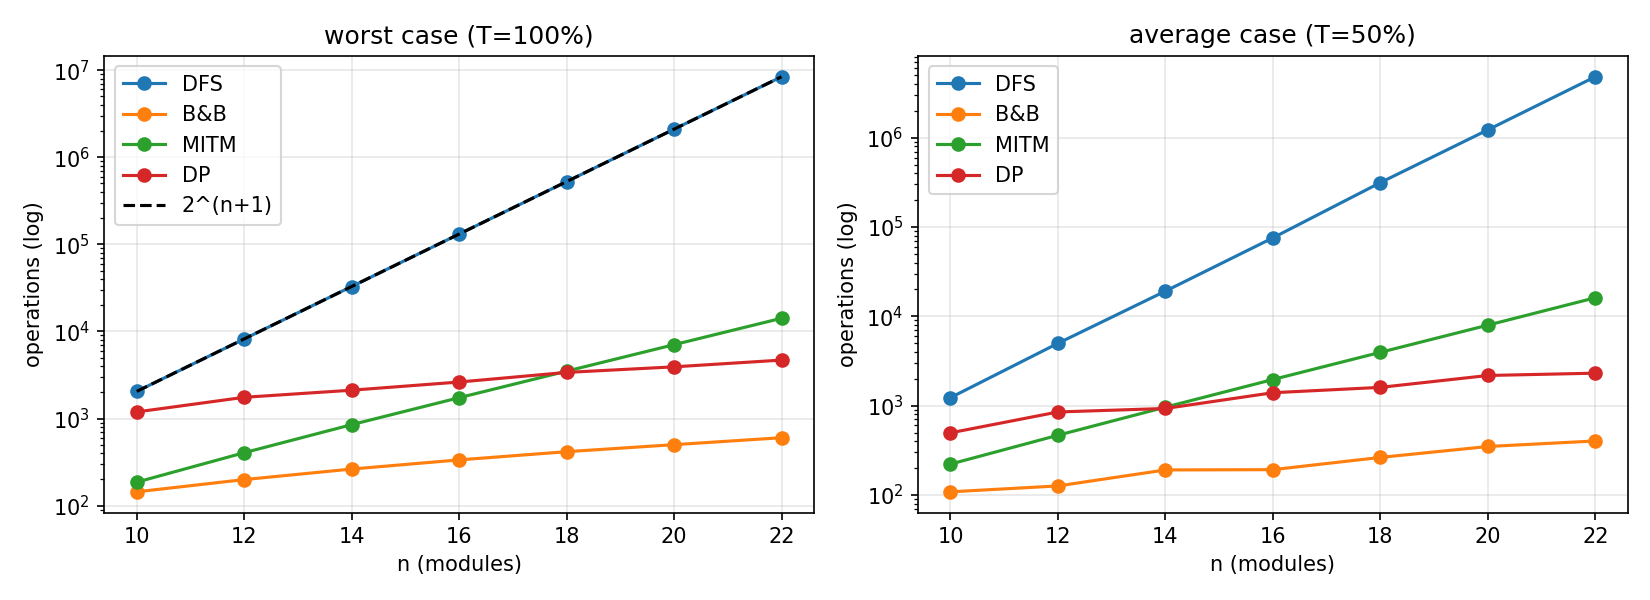
\includegraphics[width=\linewidth]{figures/fig_operations_vs_n.png}
\caption{Operations versus $n$ (log scale). The DFS follows $2^{n+1}-1$ in the worst case (left) and has the same exponential trend in the average case (right); DP, Branch and Bound and Meet-in-the-Middle grow much more slowly in this range.}\label{fig:ops-vs-n}
\end{figure}

\begin{figure}[h]
\centering
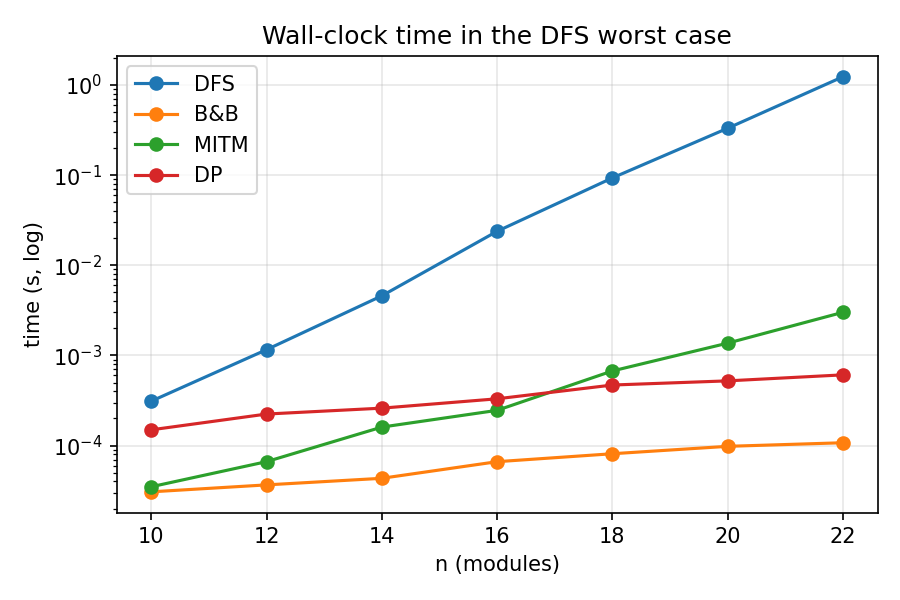
\includegraphics[width=0.62\linewidth]{figures/fig_time_vs_n.png}
\caption{Wall-clock time versus $n$ in the DFS worst case (log scale).}\label{fig:time-vs-n}
\end{figure}

In this range the DP is comparatively expensive in operations for small $n$ (its cost is $n(T+1)$ regardless of the data), while Branch and Bound needs very few operations: even in the DFS worst case it performs only 602 operations at $n=22$, because when every module fits the greedy path is optimal and the bound prunes everything else. This scenario is therefore favorable to Branch and Bound; Section~\ref{sec:exp-families} shows that this does not hold for all instance families.

\subsection{Dynamic programming and greedy at scale}

The DFS cannot be run at large $n$, but the DP and the greedy can. Table~\ref{tab:scale} and Figure~\ref{fig:scale} report $n$ from 50 to 600 modules (uncorrelated family, $\rho=0.5$). The number of DP operations coincides \emph{exactly} with $n(T+1)$ at every size, confirming Theorem~\ref{thm:dp}. The DP solves an instance with 600 modules and $T=3{,}060$ time units in about 0.37~s of pure Python, i.e.\ roughly 0.2~$\mu$s per cell. The vector version is about 40\% faster because it avoids allocating the table. The greedy performs between 0.95 and 0.98 operations per $n\log_2 n$, as expected from Proposition~\ref{prop:greedy-time}, and takes less than two milliseconds.

\begin{table}[h]
\centering
\caption{DP and greedy at scale (uncorrelated family, $R=20$, $\rho=0.5$).}\label{tab:scale}
\footnotesize\setlength{\tabcolsep}{4pt}
\begin{tabular}{@{}r r r r r r r r@{}}
\toprule
$n$ & $T$ & DP ops $=n(T+1)$ & DP time (s) & DP-vector (s) & Greedy ops & Greedy ops$/(n\log_2 n)$ & Greedy (s)\\
\midrule
50 & 273 & 13,700 & 0.0017 & 0.0010 & 269 & 0.95 & 0.0001\\
100 & 528 & 52,900 & 0.0081 & 0.0053 & 636 & 0.96 & 0.0002\\
200 & 1,097 & 219,600 & 0.0369 & 0.0247 & 1,486 & 0.97 & 0.0004\\
400 & 1,991 & 796,800 & 0.1396 & 0.0924 & 3,354 & 0.97 & 0.0011\\
600 & 3,060 & 1,836,600 & 0.3697 & 0.2230 & 5,400 & 0.98 & 0.0016\\
\bottomrule
\end{tabular}

\end{table}

\begin{figure}[h]
\centering
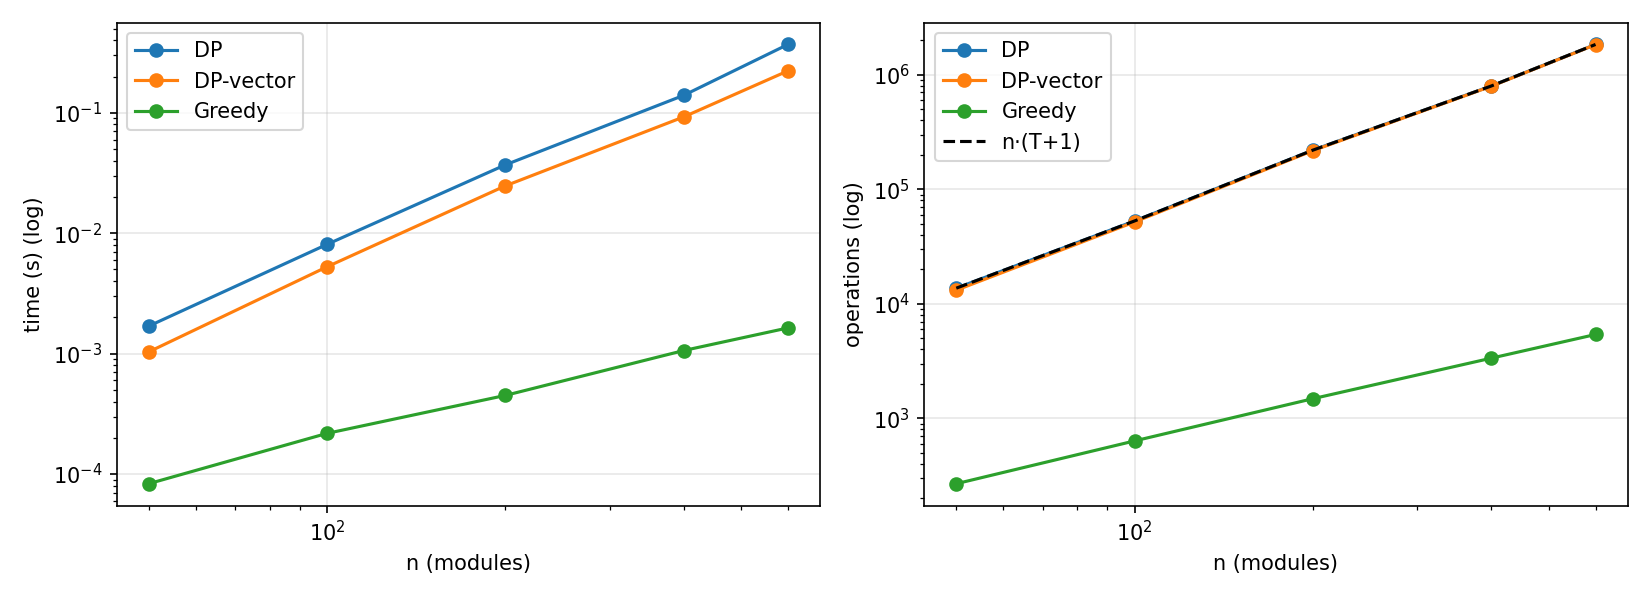
\includegraphics[width=\linewidth]{figures/fig_scale.png}
\caption{Time and operations of the DP and the greedy as $n$ grows (log--log). The dashed line is $n(T+1)$, which the DP operation count matches exactly.}\label{fig:scale}
\end{figure}

\subsection{Pseudo-polynomial behavior}

To demonstrate Proposition~\ref{prop:pseudo} we keep the same 18 modules and multiply all times and the budget by a factor from 1 to 1,024 (for instance, hours expressed in minutes and then in smaller units). The structure of the instance does not change, only the \emph{magnitude} of $T$, which goes from 100 to 102,400. Table~\ref{tab:pseudo} and Figure~\ref{fig:pseudo} show that the DP operations grow in proportion to $T$ (from 1,818 to 1,843,218, a factor of about 1,014 for a factor of 1,024 in $T$) and its time from 0.0002~s to 0.27~s, whereas the DFS, Branch and Bound, Meet-in-the-Middle and greedy counts do not change at all: they depend on $n$ and not on $T$.

\begin{table}[h]
\centering
\caption{Effect of the magnitude of $T$ ($n=18$ fixed; times and budget multiplied by the factor).}\label{tab:pseudo}
\small
\begin{tabular}{@{}r r r r r r r r@{}}
\toprule
Factor & $T$ & DP ops & DP time (s) & DFS ops & B\&B ops & MITM ops & Greedy ops\\
\midrule
$\times1$ & 100 & 1,818 & 0.0002 & 313,216 & 265 & 4,005 & 74\\
$\times4$ & 400 & 7,218 & 0.0009 & 313,216 & 265 & 4,005 & 74\\
$\times16$ & 1,600 & 28,818 & 0.0038 & 313,216 & 265 & 4,005 & 74\\
$\times64$ & 6,400 & 115,218 & 0.0153 & 313,216 & 265 & 4,005 & 74\\
$\times256$ & 25,600 & 460,818 & 0.0662 & 313,216 & 265 & 4,005 & 74\\
$\times1024$ & 102,400 & 1,843,218 & 0.2657 & 313,216 & 265 & 4,005 & 74\\
\bottomrule
\end{tabular}

\end{table}

\begin{figure}[h]
\centering
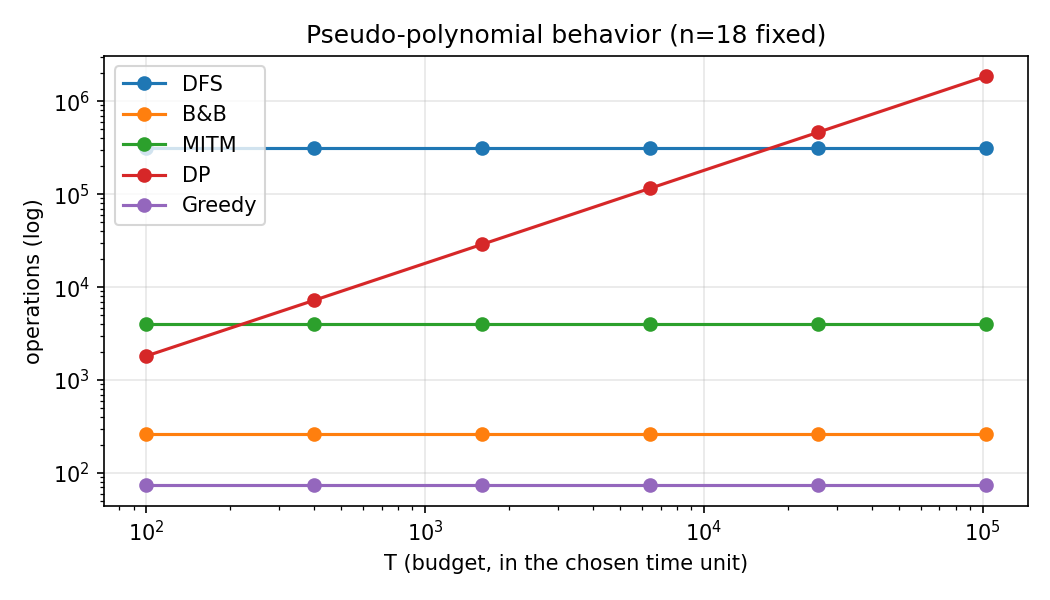
\includegraphics[width=0.75\linewidth]{figures/fig_pseudopolynomial.png}
\caption{Operations versus $T$ for fixed $n=18$ (log--log). Only the DP grows with $T$.}\label{fig:pseudo}
\end{figure}

\subsection{Quality of the greedy heuristic}\label{sec:exp-greedy}

Table~\ref{tab:quality} reports the mean and the worst gap of the greedy and of the greedy with the best single module over 30 instances per cell, for $\rho=0.3$; Figure~\ref{fig:quality} shows the gap as a function of the budget and of $n$.

\begin{table}[h]
\centering
\caption{Gap with respect to the optimum, $\rho=0.3$ (30 instances per row, $R=20$).}\label{tab:quality}
\small
\begin{tabular}{@{}r l r r r r@{}}
\toprule
$n$ & Family & Greedy mean gap & Greedy max gap & Greedy+item mean & Greedy+item max\\
\midrule
8 & Uncorrelated & 1.8\% & 10.8\% & 1.8\% & 10.8\%\\
8 & Weakly corr. & 5.5\% & 25.9\% & 5.4\% & 24.0\%\\
8 & Strongly corr. & 7.0\% & 19.0\% & 7.0\% & 19.0\%\\
\midrule
15 & Uncorrelated & 1.7\% & 9.1\% & 1.7\% & 9.1\%\\
15 & Weakly corr. & 2.7\% & 8.9\% & 2.7\% & 8.9\%\\
15 & Strongly corr. & 3.2\% & 7.9\% & 3.2\% & 7.9\%\\
\midrule
30 & Uncorrelated & 0.4\% & 2.8\% & 0.4\% & 2.8\%\\
30 & Weakly corr. & 1.0\% & 3.6\% & 1.0\% & 3.6\%\\
30 & Strongly corr. & 2.2\% & 4.6\% & 2.2\% & 4.6\%\\
\midrule
60 & Uncorrelated & 0.5\% & 1.8\% & 0.5\% & 1.8\%\\
60 & Weakly corr. & 0.2\% & 0.9\% & 0.2\% & 0.9\%\\
60 & Strongly corr. & 0.8\% & 2.2\% & 0.8\% & 2.2\%\\
\bottomrule
\end{tabular}

\end{table}

\begin{figure}[h]
\centering
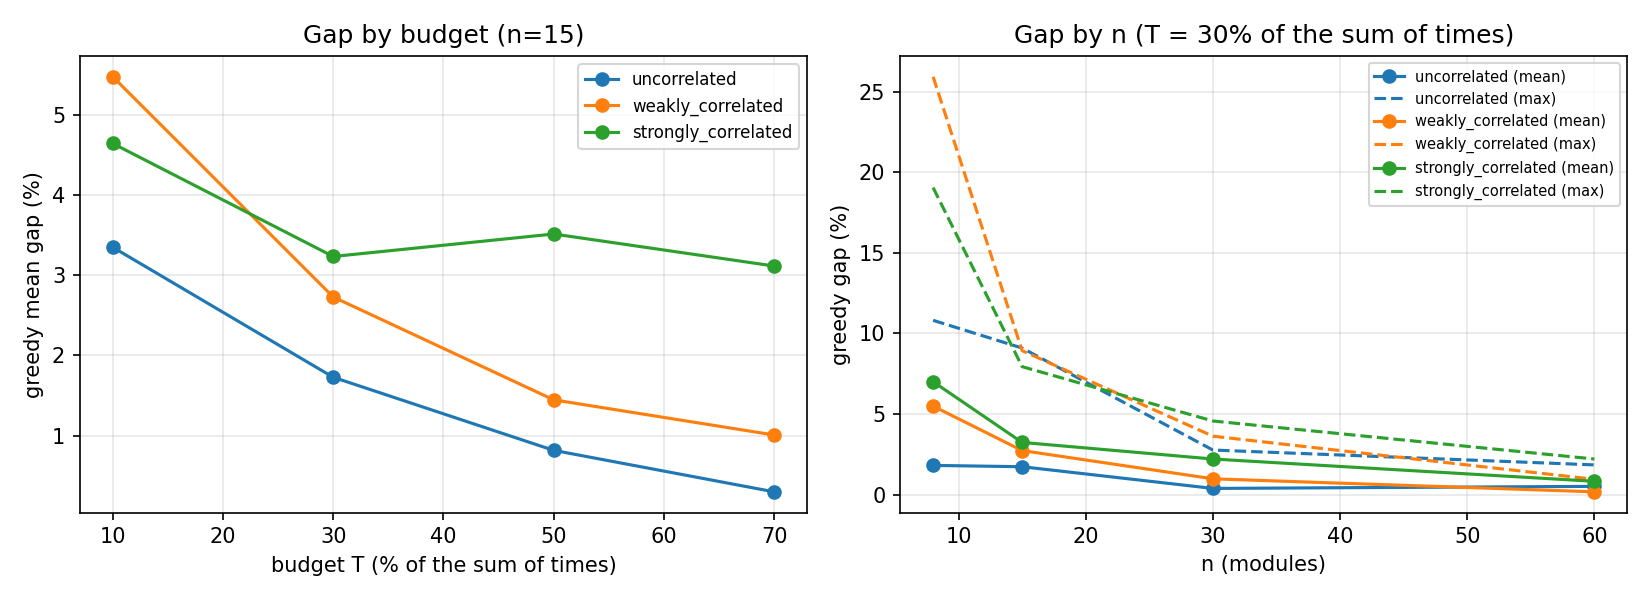
\includegraphics[width=\linewidth]{figures/fig_greedy_quality.png}
\caption{Mean gap of the greedy by budget ratio ($n=15$, left) and mean and maximum gap by $n$ ($\rho=0.3$, right).}\label{fig:quality}
\end{figure}

Three observations follow. First, the \emph{mean} gap is small and decreases with $n$: with many modules that are small relative to the budget, the greedy is nearly optimal (for instance, 0.8\% on the strongly correlated family at $n=60$). Second, the \emph{worst} gap is much larger, especially with few modules (25.9\% at $n=8$ for $\rho=0.3$, and 54.5\% at $\rho=0.1$, Table~\ref{tab:quality-item}), and it reaches 99.8\% on the adversarial instance of Section~\ref{sec:testinstance}: a small average gap offers no guarantee. Third, at $\rho=0.3$ the strongly correlated family yields the largest mean gap for every $n$ tested, in agreement with the intuition that short modules with high ratio block longer modules that are worth more; the ordering is not universal, though (at $\rho=0.1$ and $n=15$ the weakly correlated family is slightly worse, 5.5\% against 4.6\%).

\begin{table}[h]
\centering
\caption{Effect of adding the best single module to the greedy, $\rho=0.1$ (30 instances per row).}\label{tab:quality-item}
\small
\begin{tabular}{@{}r l r r r r@{}}
\toprule
$n$ & Family & Greedy mean gap & Greedy max gap & Greedy+item mean & Greedy+item max\\
\midrule
8 & Uncorrelated & 2.5\% & 50.0\% & 0.0\% & 0.0\%\\
8 & Weakly corr. & 6.7\% & 54.5\% & 0.8\% & 12.5\%\\
8 & Strongly corr. & 7.1\% & 35.0\% & 1.1\% & 11.1\%\\
\midrule
15 & Uncorrelated & 3.4\% & 23.1\% & 3.4\% & 23.1\%\\
15 & Weakly corr. & 5.5\% & 19.0\% & 5.0\% & 19.0\%\\
15 & Strongly corr. & 4.6\% & 14.6\% & 4.6\% & 14.6\%\\
\bottomrule
\end{tabular}

\end{table}

Table~\ref{tab:quality-item} shows what the variant of Proposition~\ref{prop:greedy-half} does in practice. With tight budgets and few modules, where a single module nearly fills the knapsack, it repairs the worst cases (for $n=8$, the mean gap on the weakly correlated family falls from 6.7\% to 0.8\% and the worst gap from 54.5\% to 12.5\%). For $n=15$ it brings practically no improvement, and at $\rho=0.3$ almost none for any $n$ tested (Table~\ref{tab:quality}), so the main benefit of the variant is the guarantee, not the average quality.

\subsection{Exact algorithms across instance families}\label{sec:exp-families}

Table~\ref{tab:families} and Figure~\ref{fig:families} compare Branch and Bound, Meet-in-the-Middle and the DP on uncorrelated and strongly correlated instances with $R=1000$ (so that the budget is large, which is the regime in which the DP is most expensive), $\rho=0.5$, five instances per row.

\begin{table}[h]
\centering
\caption{Operations of the exact algorithms by family ($R=1000$, $\rho=0.5$, 5 instances per row).}\label{tab:families}
\small
\begin{tabular}{@{}l r r r r r@{}}
\toprule
Family & $n$ & B\&B mean & B\&B max & MITM & DP\\
\midrule
Uncorrelated & 20 & 428 & 690 & 8,028 & 95,070\\
Uncorrelated & 30 & 683 & 834 & 261,460 & 211,032\\
Uncorrelated & 40 & 1,377 & 2,087 & 8,387,202 & 389,768\\
\midrule
Strongly corr. & 20 & 6,596 & 26,368 & 8,028 & 95,070\\
Strongly corr. & 30 & 7,655 & 16,935 & 261,460 & 211,032\\
Strongly corr. & 40 & 17,162 & 44,475 & 8,387,202 & 389,768\\
\bottomrule
\end{tabular}

\end{table}

\begin{figure}[h]
\centering
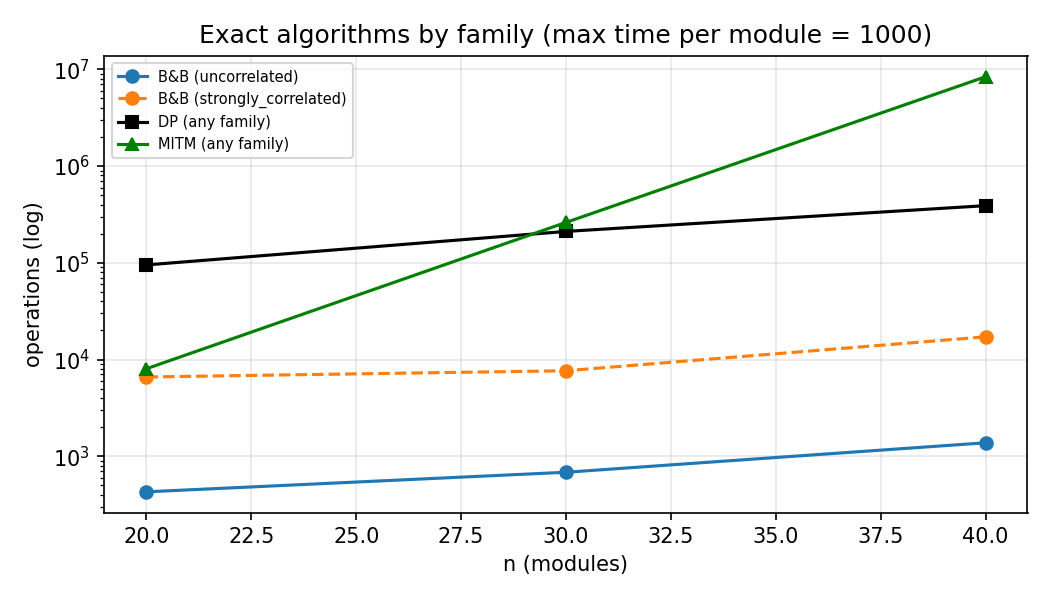
\includegraphics[width=0.75\linewidth]{figures/fig_exact_by_family.png}
\caption{Mean operations by $n$ for Branch and Bound on two families, compared with the DP and Meet-in-the-Middle (which do not depend on the family).}\label{fig:families}
\end{figure}

DP and Meet-in-the-Middle cost the same in both families, as predicted: their cost depends on $n$ and $T$ (DP) or on $n$ (MITM), not on the relation between times and scores. Branch and Bound, in contrast, depends strongly on the family: on strongly correlated instances it needs 11 to 15 times more operations than on uncorrelated ones (for instance 17,162 against 1,377 on average at $n=40$), and its worst observed run (44,475 operations) is 21 times its worst uncorrelated run (2,087). This agrees with the literature, where strongly correlated instances are reported as hard for branch-and-bound algorithms \cite{pisinger2005}; a plausible explanation, which we did not test, is that the fractional bound is less effective on them. Meet-in-the-Middle grows by a factor of 32 from $n=30$ to $n=40$ (261,460 to 8,387,202), exactly the factor $2^{10/2}$ predicted by Theorem~\ref{thm:mitm}, and from $n=30$ on it already costs more than the DP (21.5 times more at $n=40$) because $T$ is small relative to $2^{n/2}$.

\subsection{FPTAS}

Table~\ref{tab:fptas} compares the FPTAS with the exact DP on a strongly correlated instance with $n=30$.

\begin{table}[h]
\centering
\caption{FPTAS versus exact DP ($n=30$, strongly correlated, $R=20$, $\rho=0.5$).}\label{tab:fptas}
\small
\begin{tabular}{@{}l r r r r@{}}
\toprule
Algorithm & $\varepsilon$ & Score & Score / optimum & Operations\\
\midrule
exact DP & --- & 365 & 1.0000 & 4,680\\
FPTAS & 0.5 & 365 & 1.0000 & 36,690\\
FPTAS & 0.2 & 365 & 1.0000 & 91,680\\
FPTAS & 0.1 & 365 & 1.0000 & 183,330\\
FPTAS & 0.05 & 365 & 1.0000 & 366,630\\
\bottomrule
\end{tabular}

\end{table}

The FPTAS reaches the optimum in every case (ratio 1.0000, far better than the guaranteed $1-\varepsilon$), but at a high cost: it performs 7.8 times more operations than the exact DP with $\varepsilon=0.5$ and 78 times more with $\varepsilon=0.05$. The operation count grows in proportion to $1/\varepsilon$ (a factor of about 2.5, 2.0 and 2.0 as $\varepsilon$ goes from 0.5 to 0.2, 0.1 and 0.05), in agreement with Theorem~\ref{thm:fptas}. With a small $T$, approximating is more expensive than solving exactly; the FPTAS pays off only when $T$ is so large that $n(T+1)$ exceeds $n^3/\varepsilon$.

\subsection{The article's DFS on a prerequisite graph}\label{sec:exp-graph}

Finally, \code{dfs\_paths} was executed on a complete DAG (an edge from $i$ to every $j>i$), the worst case for the strategy of the article. Table~\ref{tab:graph} shows that the number of generated paths is exactly $2^{n-1}$ for every $n$ tested (32,768 paths for $n=16$), as derived in Section~\ref{sec:design}: the exhaustive path enumeration of the article is exponential in the size of the course graph.

\begin{table}[h]
\centering
\caption{Paths generated by the prerequisite-graph DFS on a complete DAG.}\label{tab:graph}
\small
\begin{tabular}{@{}r rrrrrrr@{}}
\toprule
$n$ & 4 & 6 & 8 & 10 & 12 & 14 & 16\\
\midrule
Paths generated & 8 & 32 & 128 & 512 & 2,048 & 8,192 & 32,768\\
$2^{n-1}$ & 8 & 32 & 128 & 512 & 2,048 & 8,192 & 32,768\\
\bottomrule
\end{tabular}

\end{table}
